\frametitle{Research Motivation}

\begin{columns}[T]

%=====================================================================
% left: the picture -- one problem at the intersection of three fields
%=====================================================================
\begin{column}{0.48\textwidth}
\centering
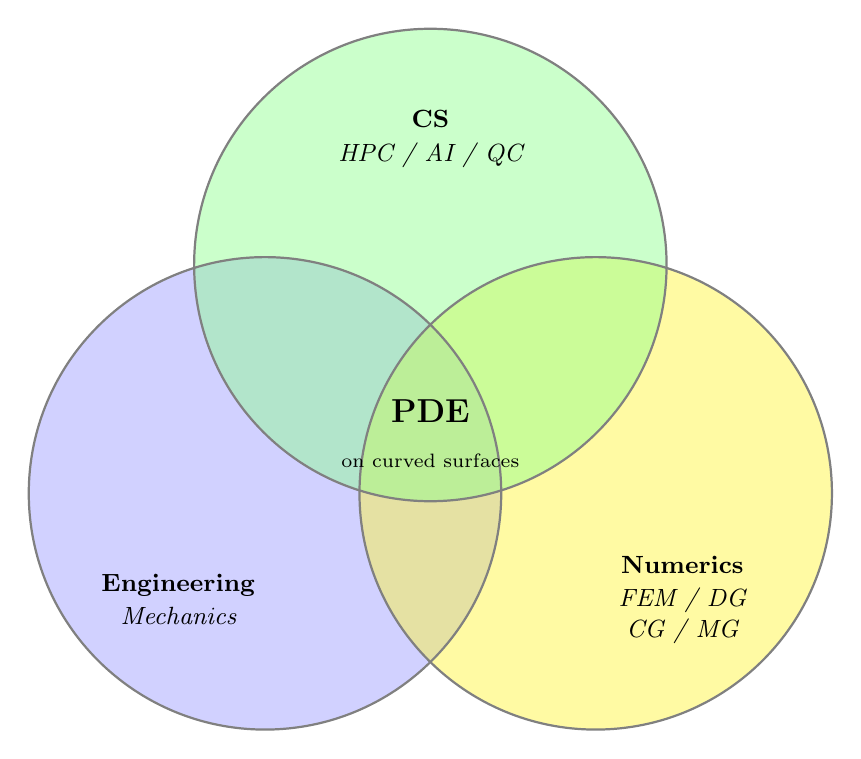
\begin{tikzpicture}
  % ---- the three fields: the overlaps come from compositing the fills ----
  \begin{scope}[opacity=0.45]
    \fill[blue!40]   (-2.1,0)   circle (3.0);
    \fill[yellow!80] ( 2.1,0)   circle (3.0);
    \fill[green!45]  ( 0.0,2.9) circle (3.0);
  \end{scope}
  \begin{scope}[draw=black!50, thick]
    \draw (-2.1,0)   circle (3.0);
    \draw ( 2.1,0)   circle (3.0);
    \draw ( 0.0,2.9) circle (3.0);
  \end{scope}

  % ---- each label sits in the region exclusive to its own field ----
  \node[align=center, font=\small] at (-3.20,-1.35)
       {\textbf{Engineering}\\[1pt]\itshape Mechanics};
  \node[align=center, font=\small] at ( 3.20,-1.35)
       {\textbf{Numerics}\\[1pt]\itshape FEM / DG\\\itshape CG / MG};
  \node[align=center, font=\small] at ( 0.00, 4.50)
       {\textbf{CS}\\[1pt]\itshape HPC / AI / QC};

  % ---- the intersection, which is where this thesis sits ----
  \node[align=center, font=\large\bfseries] at (0,1.05) {PDE};
  \node[align=center, font=\scriptsize]     at (0,0.42) {on curved surfaces};
\end{tikzpicture}
\end{column}

%=====================================================================
% right: the loop that structures the whole thesis
%=====================================================================
\begin{column}{0.52\textwidth}
\small

The thesis sits where the three fields meet: a classical engineering problem,
solved by numerical methods, accelerated with modern computing.

\vspace{0.5em}
{\centering
\begin{tikzpicture}[
    every node/.style={font=\small, align=center},
    q/.style={draw, rounded corners=2pt, fill=blue!8, draw=blue!45,
              inner sep=6pt, text width=105mm, minimum height=9mm},
    ar/.style={-{Latex[length=2mm]}, line width=0.7pt, draw=black!65},
  ]
  \node[q] (q1) {\textbf{Can I solve it?}};
  \node[q, below=6mm of q1] (q2)
       {\textbf{Can I measure the error?}\\[2pt]
        {\scriptsize and so say how far the result can be believed}};
  \node[q, below=6mm of q2] (q3) {\textbf{Can I speed it up?}};
  \node[q, below=6mm of q3] (q4)
       {\textbf{Have I used every effort available}\\[2pt]
        \textbf{for a practical problem?}};
  \draw[ar] (q1) -- (q2);
  \draw[ar] (q2) -- (q3);
  \draw[ar] (q3) -- (q4);
\end{tikzpicture}\par}

\vspace{0.4em}
Both pipelines compared in this talk are put through the \alert{same loop}.
Chapter~1 states it as \alert{six precise research questions}.
\end{column}

\end{columns}
